\documentclass[conference]{IEEEtran}
\IEEEoverridecommandlockouts
% The preceding line is only needed to identify funding in the first footnote. If that is unneeded, please comment it out.
\usepackage{cite}
\usepackage{amsmath,amssymb,amsfonts}
\usepackage{algorithmic}
\usepackage{graphicx}
\usepackage{textcomp}
\usepackage{xcolor}
\usepackage{pgfplots}
\pgfplotsset{compat=1.18}

\def\BibTeX{{\rm B\kern-.05em{\sc i\kern-.025em b}\kern-.08em
    T\kern-.1667em\lower.7ex\hbox{E}\kern-.125emX}}
\begin{document}

\title{Video License Plate Parking System}

\author{\IEEEauthorblockN{Dominik Schweigl}
\and
\IEEEauthorblockN{Daniel Wenger}
\and
\IEEEauthorblockN{Nikola Adzic}
}

\maketitle

\section{Introduction}
Efficient parking management is an increasingly important challenge in urban environments, where traditional ticket-based parking systems often lead to congestion at entry and exit points, operational overhead, and poor user experience due to lost tickets and limited real-time visibility into parking availability.

This project presents a distributed, ticketless parking system based on automatic license plate recognition. Cameras installed at parking lot entry and exit points capture vehicle license plates, which serve as the identifier for access control and payment. This enables vehicles to enter and exit without physical tickets or manual interaction.
Users interact with the system through a single web application, accessible both on smartphones and on on-site payment stations, which allows them to pay, reserve parking spaces, view parking space availability, and discover the nearest parking facilities based on their location.

This work focuses on the system architecture, communication patterns, 
and deployment considerations of the distributed parking solution. 
Physical devices such as cameras, gates, and traffic lights are 
simulated, and license plate recognition is implemented using a 
YOLO license plate detection model combined with the EasyOCR optical character recognition model without evaluation 
of computer vision performance.

The remainder of this paper is structured as follows. Section~\ref{sec:system_architecture}
describes the overall system architecture and its main components. 
Section~\ref{sec:implementation_details} details the implementation 
of the edge, cloud, and web layers. Section~\ref{sec:evaluation} evaluates the system 
under different load scenarios. Section~\ref{sec:limitations} discusses 
the limitations of our system, and Section~\ref{sec:conclusion} summarizes the paper and outlines future work.

\section{System Architecture}
\label{sec:system_architecture}

The proposed parking system adopts a distributed edge--cloud architecture, 
organizing responsibilities across four distinct layers. The IoT layer 
handles sensing and actuation, the edge layer manages real-time processing 
and actuator control, the cloud layer provides centralized services for 
information management, booking, and payments, and the presentation layer 
enables user interaction through a web-based interface. This layered approach 
ensures low-latency parking actuator control at parking facilities while 
supporting centralized payment processing and a global view of parking 
availability. Figure~\ref{fig:architecture_diagram} illustrates the system 
components and their interactions. For simplicity, only a single parking 
lot is shown, though each facility deploys its own identical edge configuration.

\begin{figure}[t]
    \centering
    \includegraphics[width=1\linewidth]{assets/architecture_diagram.png}
    \caption{
        The architecture diagram for this project. For clarity, only 
        one parking lot edge is shown. Each parking lot has its own 
        edge server, gate, camera, and message queue.    
    }
    \label{fig:architecture_diagram}
\end{figure}

\subsection{Edge Layer}

Each parking lot is equipped with an edge server that is directly connected 
to the physical infrastructure of the facility. This includes two cameras 
positioned at the entry and exit gates, barrier gates, and traffic lights. 
The cameras continuously stream video data to the edge server via a local 
NATS message queue, which decouples video producers from consumers. 

The edge server performs real-time license plate detection on incoming video 
frames using a YOLO license plate detection model combined with the EasyOCR optical character recognition model. 
When a vehicle is detected at the 
entry gate, 
the edge server registers the vehicle locally and issues a command via the local
NATS message queue to open 
the entry barrier actuator. Local persistence using an SQLite database is maintained 
to ensure data robustness against temporary edge server failures.

At the exit gate, the edge server again detects the vehicle's license plate 
and queries the cloud backend to verify the payment status associated with 
the plate. If the vehicle has paid and the allowed exit window has not 
expired, the edge server opens the exit gate and signals a green traffic 
light. Otherwise, the gate remains closed and a red signal instructs the 
driver to return and complete payment. In addition, the edge server sends
occupancy updates to the cloud every time a vehicle enters or exits the parking lot.

\subsection{Cloud Layer}

The cloud backend is hosted on Amazon EC2 and implemented using the Akka 
framework. It serves as the central coordination point for all parking 
facilities. The cloud maintains global state such as parking lot registrations, 
current occupancy levels, payment status, and advances bookings to the
respective edge servers. Each parking 
lot periodically reports its current occupancy to the cloud, allowing the 
backend to maintain an up-to-date view of available parking spaces across 
all facilities.

The Communication between edge servers and the cloud backend uses a combination 
of synchronous and asynchronous mechanisms. REST-based HTTP endpoints exposed 
via Akka HTTP are used for operations from the edge to the cloud since many
operations need immediate responses, such as payment verification at exit gates. 
Asynchronous messaging via a 
NATS message queue hosted on it's own EC2 instance is used for event-driven interactions, such as propagating 
booking requests from the cloud to the appropriate edge server.


\subsection{Web and User Interaction Layer}

User interaction with the system is provided through a web application
implemented using React and hosted 
on a separate EC2 instance using Nginx as a web server. The same web 
application is accessible both from users' personal smartphones and from 
on-site payment stations within parking facilities. Through this interface, 
users can view available parking lots, reserve parking spaces in advance using 
their license plate number, complete payments, and discover nearby parking 
facilities based on their current location.

\section{Implementation details}
\label{sec:implementation_details}

This section presents the implementation of the system across its various 
layers, including the IoT components, edge server, cloud backend, and web 
interface. For each layer, the chosen design and implementation decisions 
are explained and justified.


\subsection{IoT Implementation}

The IoT components of the parking lot system are implemented in Python 
and deployed using Docker containers with \texttt{docker-compose}, ensuring 
that the system is independent of the underlying execution infrastructure. 
Both the camera simulations and actuator interfaces run inside these 
containers.

\paragraph{Camera}
The entry and exit points of the parking lot are simulated by two camera 
streams, which alternately transmit images from a car license plate detection 
dataset and a reference empty street scene. 
The dataset we use is the Car License Plate Detection dataset from 
Kaggle. It features more than 400 images of car front/ rear views 
with clearly visible license plates. We chose a subset of the 50 most clearly
visible license plates for our simulation.

Images are published to an edge server via a NATS message queue via the 
camera simulation python script to two separate message queue subjects. 
It is made sure that the data sent 
by the entry and exit camera streams is consistent. This means that the exit 
camera will only show cars leaving that have previously entered. The 
duration of the cars inside the car parks is sampled randomly.

Cars enter the lot at a steady pace, with one car added every two display cycles of 3 seconds (\texttt{FRAME\_DELAY}), yielding an average entry rate of
\[
R_\text{entry} = \frac{1}{2 \cdot \text{FRAME\_DELAY}} \approx 0.166 \text{ cars/second}.
\]
Each car has a probability of leaving the lot in any given frame of
\[
P_\text{exit} = \frac{1}{4 \cdot \text{FRAME\_DELAY}} \approx 0.0833 \; (8.33\%),
\]
corresponding to an average exit rate of
\[
R_\text{exit} = \frac{P_\text{exit}}{\text{FRAME\_DELAY}} \approx 0.028 \text{ cars/second}.
\]
This setup results in a parking lot that gradually fills over time, with entries initially outpacing exits.

\paragraph{Parking Lot Gates and Traffic Light Interface}
The parking lot gates and traffic lights are simulated via a web-based 
interface implemented using \texttt{FastAPI}. The framework was selected 
due to its support for rapid and intuitive development. In addition, 
FastAPI provides native support for asynchronous 
communication and WebSockets, which makes it well suited for real-time 
IoT applications.

The interface provides a live view of the current state of all actuators 
for each parking lot individually. It receives continuous state updates 
from the edge server through the local NATS message broker, ensuring that 
changes in actuator states, such as barrier positions or traffic light 
signals, are reflected on the web dashboard. Furthermore, the 
interface displays the camera streams from the entry and exit points, 
which allows to visually monitor the camera streams and correlate actuator 
behavior with observed traffic conditions.

\subsection{Edge Implementation}

The edge server is responsible for all real-time processing at the parking 
lot gates. For each incoming camera frame, it executes a YOLOv11-based license 
plate detection pipeline followed by optical character recognition (OCR) to 
extract the license plate text. All detections are processed locally at the 
edge without requiring immediate interaction with the cloud. This design 
keeps network traffic to the cloud low and
ensures low-latency actuator control and allows the system to remain 
operational during temporary cloud disconnections, though with some limitations 
at the exit gate due to synchronous payment verification at the cloud. The edge server is 
implemented in Python, as the employed machine learning models and inference 
pipelines are exclusively available through Python-based frameworks.

To maintain local state, the edge server uses a lightweight SQLite database. 
SQLite was selected for its low operational overhead, zero-configuration 
deployment, and suitability for resource-constrained edge environments. As 
an embedded database, it runs within the application process and requires no 
separate database service, providing sufficient performance for handling 
several hundred concurrent parking sessions per lot while keeping the system 
simple.

When a vehicle appears at the entry point, the edge server checks whether an 
active session for the same license plate already exists and only creates a 
new record if the vehicle is not already inside the parking lot. This prevents 
duplicated entries caused by repeated detections of the same vehicle while it 
remains in front of the entry camera. For exit events, the edge queries the cloud 
service to verify the payment status, retrieves the corresponding local 
session from SQLite, and completes it by recording the exit timestamp.

Communication between the camera streams, actuator controllers, and the edge 
server is handled using NATS as the message broker. NATS was selected for its 
lightweight architecture, low-latency message delivery, and minimal operational 
overhead, making it well suited for deployment on resource-constrained edge 
servers. In contrast to heavier brokers such as Apache Kafka or RabbitMQ, which 
emphasize message persistence and complex broker management, NATS is optimized 
for real-time, transient messaging patterns while the throughput and provides 
ample throughput to reliably handle the modest message rates in the low tens 
generated by the camera streams and actuator commands.

Using NATS creates a clean decoupling between data producers (camera streams) 
and consumers (edge processing and actuator controllers).
The camera streams publish data using NATS core publish--subscribe semantics, 
where messages are delivered on a best-effort basis only to currently active 
subscribers and are not persistently stored. This behavior aligns with the 
nature of camera frames, which are only relevant at the time of generation 
and have no value if processed later. By avoiding message persistence, the 
system reduces memory and storage overhead while ensuring timely delivery of 
live camera data. Actuator commands and state updates similarly benefit from 
this low-latency, ephemeral communication model, enabling responsive and 
reliable gate control at the edge.



\subsection{Cloud Implementation}


Regarding our Service choices, the Akka Framework is used in the Cloud 
Layer as it is mandatory for this assignment. Actors will store their 
state in a DynamoDB table because we want to ensure reliability even if 
some server with Akka Actors crashes. The communication from the cloud 
to the edge server is done through a message queue to make the edge 
server location transparent for the cloud. The edge server computes 
the detection algorithm on the video stream and manages the local IoT 
devices as well as parking data to keep network traffic to the cloud 
low. This way we only send small messages of detection events with 
current open capacity to the cloud. Communication from the edge to 
the cloud Akka Backend does not go through the message queue and 
instead uses Akka's HTTP REST API. This is because some of the 
calls to the cloud for information retrieval like a GET request 
for car payment status fit better as synchronous calls rather 
than asynchronous messages. Therefore, to have a uniform access 
point for the edge we will use the REST API also for capacity 
update events. Though we leave the possibility open to also use 
the message queue for communication from the edge to the cloud backend.

(Akka HTTP) : Edge servers need synchronous immediate responses for certain operations,
    such as verifying payment status at exit gates or retrieving the list of registered parking lots. For these interactions, we implemented a RESTful HTTP API using Akka HTTP. Edge servers send HTTP requests to specific endpoints exposed by the cloud backend, which processes them and returns appropriate responses. This approach provides a uniform access point for edge servers and web clients alike.
    Cloud needs to be available at all times for the system to work anyways.

In the cloud layer we rely on Akka Typed as the central orchestration mechanism for all parking-lot related functionality. An embedded Akka HTTP server runs within the same typed ActorSystem and exposes a synchronous API to edge servers. Internally, the system is entirely message-driven, which gives us clear separation of concerns, robust concurrency, and predictable error handling.

At the core sits a typed ParkingLotManager actor that maintains the registry of parking lots and supervises one ParkingLot actor per lot. The manager accepts commands to register and deregister lots, to update occupancy, and to fetch either the status of a specific lot or the complete set of registered lots. Each ParkingLot actor keeps the local state for a single lot, namely current occupancy and maximum capacity, and derives the number of available spaces from those. Occupancy updates are handled as fire-and-forget messages to minimize latency, while status queries are served synchronously using Akka’s ask pattern with typed timeouts to provide deterministic responses.

Payments are handled by a dedicated typed Payment actor that tracks a parking session per license plate. When a car is recorded as having entered, the actor creates or updates the session with the entry time. A payment command marks the session as paid and computes the price based on the parking duration using a simple policy with half-hour increments. At exit, the actor can be asked synchronously to verify whether the car has paid and to return the current price; once the car leaves, the session is deleted to ensure that only currently parked cars are stored.

Bookings are mediated by a typed Booking actor that acts as the cloud-side gateway to the edge servers. When a booking is created through the API, the actor publishes a JSON message containing an action field set to “book” and the license plate to a parking-lot specific NATS subject, which the corresponding edge server subscribes to. When a booking is cancelled, the actor similarly publishes an action “cancel” message. This approach intentionally keeps booking state lightweight in the cloud and delegates the effective reservation and occupancy adjustments to the edge, where the real-world constraints and device control live.

The HTTP API mirrors these responsibilities in a small set of endpoints. Parking-lot management includes an endpoint to register lots, one to deregister, a status endpoint to retrieve current occupancy and capacity, and an endpoint to list all registered lots. Occupancy updates are accepted via a simple POST call and relayed to the appropriate ParkingLot actor without awaiting a reply. The payment flow provides endpoints to record entry, to mark a license plate as paid and return the computed price, to check payment status at the exit, and to delete the session after successful departure. Bookings are exposed through a POST endpoint to create a booking and a DELETE endpoint to cancel it, both of which result in the Booking actor publishing the appropriate NATS messages to the lot-specific subject.

Communication between cloud and edge is deliberately mixed to match the semantics of each interaction. Edge-to-cloud interactions that benefit from synchronous responses—such as retrieving payment status or listing registered lots—use the HTTP API and the ask pattern under the hood. High-frequency, one-way updates—such as occupancy changes—use fire-and-forget messages for minimal overhead. Cloud-to-edge interactions for bookings use NATS publishing because reservations are asynchronous events best handled locally at the edge, and messaging scales naturally across many geographically distributed edge servers while keeping the cloud simple.

Using REST for edge-to-cloud requests provides a uniform access point for edge servers and web servers and is a natural fit for synchronous queries,
while NATS for cloud-to-edge booking events decouples producers and consumers and keeps the edge authoritative for local capacity
management. Finally, placing state where it belongs—lot occupancy inside ParkingLot actors, payment sessions inside the Payment actor,
and booking mediation inside the Booking actor—minimizes side effects and keeps responsibilities clear.

Each ParkingLot actor additionally stores static metadata describing the physical
location of the car park in the form of latitude and longitude. These coordinates
are provided during parking-lot registration and are returned as part of the lot
status via the HTTP API. This allows clients to perform distance calculations and
routing without requiring external geocoding services.

For the web application, we implemented a web application using React that allows
users to interact with the parking system. Through this application, users can
see all registered parking lots, check their current availability, reserve
a parking space in advance by entering their license plate number and pay.
We host the web application on a separate EC2 instance from the Akka backend
using Nginx as a web server.

\subsection{Web Interface}

For the web interface, we implemented a web application using React that allows
users to interact with the parking system. Through this application, users can
see all registered parking lots, check their current availability, reserve
a parking space in advance by entering their license plate number and pay. 
React was chosen for its component-based architecture, which simplifies
the development and maintenance of dynamic user interfaces.
The interface was styled using Tailwind CSS, whose utility-first approach enables
rapid creation of responsive and consistent layouts with minimal custom styling.

To help users find a suitable parking lot, the application can access the
current location of the client device using the browser's geolocation feature.
Each parking lot is provided by the backend together with its geographical
coordinates and the distance to the corresponding parking lot. The frontend
application sorts the results so that nearby
parking options are shown first. A routing button is also provided, which opens
a navigation view in an external map service for the selected parking lot.

\section{Evaluation}
\label{sec:evaluation}

\subsection{Evaluation Setup}

The cloud components of the system were deployed on Amazon Web Services 
(AWS) using Terraform to ensure reproducibility and consistency across 
experiments. The setup consists of three EC2 instances hosting the 
backend application, message broker, and web frontend, respectively. 
All instances use the \texttt{t3.micro} instance type, providing 2 
virtual CPUs and 1~GB of RAM, which is sufficient for evaluating the 
system under moderate load. The instances run Amazon Linux 2023 (x86\_64).

The backend service is deployed as a Java-based Akka application running 
on Amazon Corretto JDK~17, while the NATS message broker is hosted in a 
Docker container to facilitate lightweight and isolated operation. The 
web frontend is served via Nginx as a static application. Network access 
is controlled using a dedicated security group that exposes only the 
required ports for HTTP communication, backend APIs, NATS messaging, 
and SSH access.


\subsection{Test Case 1: Cloud Backend Load with Increasing Number of Edge Servers}

The first test case evaluates the scalability of the cloud backend when the number of connected edge servers increases. In a real deployment, multiple geographically distributed parking facilities may send frequent occupancy updates to the cloud at the same time. This test therefore focuses on how the backend behaves under increasing request load generated by multiple independent edge servers.

To isolate the cloud infrastructure, license plate detection and OCR were not part of this experiment. Instead, a custom Python-based load testing script was used to simulate edge servers that periodically send occupancy updates via the REST API.

The cloud backend was deployed on a single Amazon EC2 instance and exposed a public HTTP endpoint. For the test, ten simulated edge servers were started. Each edge sent one occupancy update per second, resulting in a steadily increasing number of concurrent HTTP requests handled by the backend. To account for request overlap, the maximum concurrency was limited to 50 parallel requests.

The test was executed with the following parameters:

\begin{itemize}
    \item Number of simulated edge servers: 10
    \item Occupancy update rate: 1 update per second per edge
    \item Test duration: 60 seconds
    \item Maximum concurrent HTTP requests: 50
    \item Request timeout: 5 seconds
\end{itemize}

In addition to occupancy updates, a small number of health check requests as well as parking-lot registration and deregistration requests were issued to ensure that the system remained responsive for management operations while under load.

During the test run, the cloud backend processed all incoming requests successfully. A total of 489 occupancy update requests were sent and acknowledged. No timeouts, client-side errors (4xx), or server-side errors (5xx) occurred throughout the experiment.

The average response time of the occupancy update endpoint was approximately 115\,ms. The median latency was around 111\,ms, while 95\% of all requests were completed in under 130\,ms. The maximum observed response time was approximately 223\,ms.

These results show that the cloud backend can handle concurrent updates from multiple edge servers with stable response times. Even under sustained load, no signs of request backlog or performance degradation were observed. This indicates that the actor-based architecture and the chosen communication pattern are well suited for coordinating multiple parking facilities in parallel.
 
To further explore the limits of the system, an additional stress run was executed
within this test case by significantly increasing the number of simulated edge
servers and the request rate. In this extreme configuration, more than 3000
requests were sent within the same time window. Under this load, all requests
exceeded the configured timeout threshold of five seconds and were recorded as
client-side timeouts. While the backend remained operational, the response times
clearly exceeded acceptable limits, revealing scalability constraints of the
single-instance deployment.

\begin{figure}[h!]
\centering
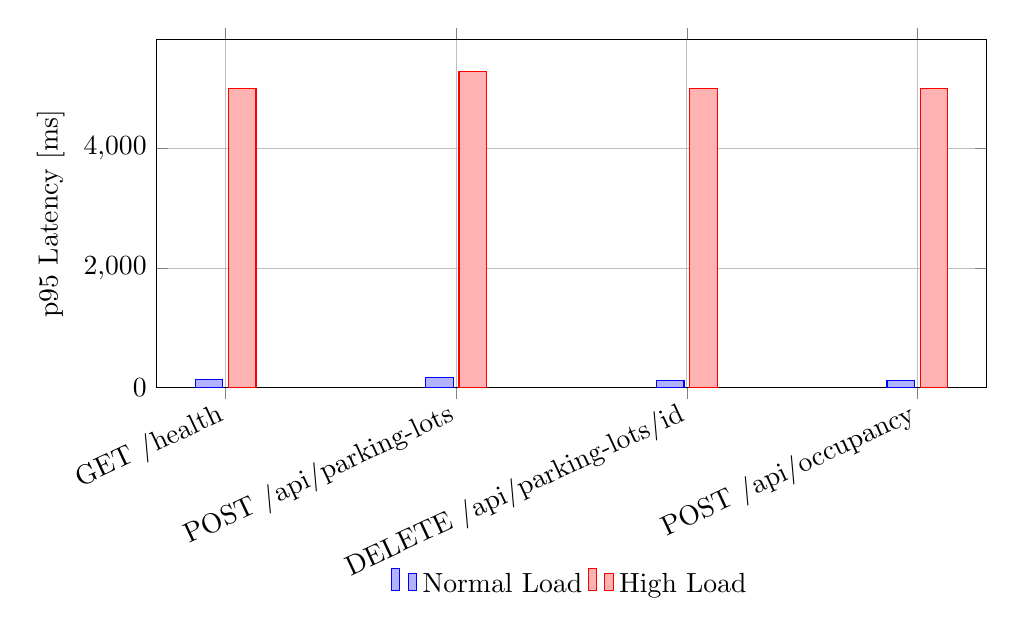
\begin{tikzpicture}
\begin{axis}[
    ybar,
    bar width=10pt,
    width=\linewidth,
    height=6cm,
    ymin=0,
    ylabel={p95 Latency [ms]},
    symbolic x coords={
        GET /health,
        POST /api/parking-lots,
        DELETE /api/parking-lots/{id},
        POST /api/occupancy
    },
    xtick=data,
    xticklabel style={rotate=25, anchor=east, yshift=-4pt},
        legend style={
            at={(0.5,-0.5)},
            anchor=north,
            legend columns=2,
            draw=none
        },
    grid=both
]

% -------- Normal Load --------
\addplot coordinates {
    (GET /health,131.19)
    (POST /api/parking-lots,171.08)
    (DELETE /api/parking-lots/{id},117.21)
    (POST /api/occupancy,125.67)
};

% -------- High Load --------
\addplot coordinates {
    (GET /health,5005.38)
    (POST /api/parking-lots,5291.17)
    (DELETE /api/parking-lots/{id},5005.37)
    (POST /api/occupancy,5005.71)
};

\legend{Normal Load, High Load}

\end{axis}
\end{tikzpicture}
\caption{HTTP backend p95 latency per endpoint under normal and high load.}
\label{fig:http_latency_comparison}
\end{figure}


\subsection{Test Case 2: Web Interface Load Test (Nginx + React)}
To evaluate the performance of the web interface, we first benchmarked the standalone web server that serves the compiled React frontend. This test was intentionally isolated from the rest of the system components, meaning that neither the Akka cloud backend nor any edge servers were involved. In this setup, the measured latency and throughput mainly reflect the capability of the Nginx server to deliver static frontend assets under concurrent access.

We used the \texttt{wrk} benchmarking tool with 4 threads and 100 concurrent connections over a duration of 60 seconds:
\begin{verbatim}
wrk -t4 -c100 -d60s http://3.87.5.60
\end{verbatim}

During the test run, the server handled a total of 54{,}162 requests, resulting in an average throughput of 901.89 requests per second. The measured average response latency was 111\,ms, while the maximum observed latency remained below 450\,ms. No failed requests or timeouts were recorded, indicating stable behaviour under this load. Overall, these results suggest that the web server is not a bottleneck for moderate concurrency and can reliably serve a high number of simultaneous users with low latency.

\textbf{High-load attempt.} We additionally attempted a more aggressive load configuration to simulate significantly higher concurrency. Under this extreme setup, the system behaviour became unstable and requests started to time out, which indicates that the current deployment is not configured to sustain such high load without additional scaling or tuning. Since this load level exceeds the expected operating range of our prototype deployment, we primarily use the moderate load test above as the main reference point for the evaluation.

\subsection{Test Case 3: NATS Publish Load Test for Edge Messaging}

In addition to the HTTP-based cloud interface and the web frontend, we evaluated the NATS messaging layer used at the edge of the system. NATS is responsible for transporting continuous camera streams and control messages between IoT devices and edge servers and is therefore critical for real-time operation.

In this test case, we measured how the NATS server handles sustained publish load without request--reply semantics. A dedicated load test client continuously published messages to the entry and exit camera subjects of a single parking lot. Each message had a payload size of approximately 150~KB, which corresponds to compressed image frames used by the simulated cameras. Messages were sent at a rate of 5 messages per second per stream over a duration of 60 seconds.

During the experiment, a total of 299 messages were published for each stream, resulting in nearly 600 published messages overall. No send errors, timeouts or missing subscribers were observed during the test. All messages were accepted by the NATS server, indicating stable operation under continuous load.

Since the camera streams are implemented as fire-and-forget publishers, no round-trip latency was measured in this test. Instead, the focus was on message throughput and delivery reliability. The results show that the NATS server can reliably handle sustained streaming traffic at the edge without message loss or instability.

Overall, this experiment confirms that NATS is well suited for continuous data streaming between IoT devices and edge servers in the proposed system. While this test does not provide latency measurements, it demonstrates that the messaging layer remains stable under realistic camera load and complements the HTTP-based load tests performed on the cloud backend.

\section{Limitations}
\label{sec:limitations}


While the implemented system covers the core functionality of a video
license plate parking system, there are several limitations to consider.

\paragraph{Payment event latency optimization}
To reduce latency at the exit gate, payment events could be propagated 
to the edge server proactively rather than queried on demand. In the 
current design, the edge server performs a synchronous request to the 
cloud backend when a vehicle approaches the exit, introducing avoidable
latency. By pushing payment status updates to the edge immediately after 
a transaction is completed, the edge system could locally cache this 
information and eliminate the need for synchronous cloud queries at 
exit time. This approach would result in faster gate responses and 
improved robustness during transient cloud disconnections.

This limitation is further emphasized by the fact that the current 
payment system is a mock implementation without integration with real 
payment gateways. In a production environment, secure payment providers 
such as Stripe or PayPal would be required to process actual financial 
transactions, inevitably introducing additional latency during payment 
verification. By proactively propagating payment status updates to the 
edge server, this added delay could be mitigated.

\paragraph{Security and authentication}
Another major limitation of the current system is the absence of 
authentication and authorization mechanisms. At present, the cloud 
backend does not verify the identity of parking lot servers during 
registration or when receiving occupancy updates, which could allow 
unauthorized entities to inject or manipulate parking lot data. A 
production--ready deployment would therefore require the introduction 
of secure authentication mechanisms, such as mutual TLS or API 
key based access control, to ensure data integrity and system security.

\paragraph{Cloud Scalability and Availability}
Another big limitation is the simplistic hosting setup. The cloud 
components, Nginx webserver, Akka backend, and NATS message broker, 
are hosted on a single EC2 instance respectively without any load balancing or 
auto-scaling.
This setup may not handle high traffic loads or provide sufficient 
fault tolerance for big systems as each of them represents a single point of failure.
In a production environment, deploying the cloud components using container 
orchestration platforms like Amazon ECS
along with load balancers and auto-scaling, would improve reliability 
and scalability.

As all communication from the cloud to the edge goes through the NATS message
broker and messages need to be temporarily stored, the need for heavier 
message brokers like Apache Kafka could be considered for better scalability
and fault tolerance. Though for the current system NATS is sufficient.

\paragraph{Cloud Scalability and Availability}
A further limitation of the current system is the simplicity of the 
cloud deployment. The cloud components—the Nginx web server, 
the Akka-based backend, and the NATS message broker—are each hosted 
on a single EC2 instance, without load balancing or automatic scaling. 
While sufficient for prototyping and evaluation, this architecture may 
not sustain high traffic volumes and offers limited fault tolerance, 
as each component constitutes a single point of failure.
Reliability and scalability could be 
significantly improved by deploying the cloud services using 
container orchestration platforms such as Amazon ECS, in combination 
with load balancers and auto-scaling mechanisms. 

Furthermore, because all cloud-to-edge communication is mediated by 
the message broker and involves temporary buffering of messages, the 
system could benefit from brokers such as Apache Kafka, which provide 
persistent storage, replication, and message replay in the event of 
consumer or broker failures. For the scale of the current system, 
however, NATS remains a suitable choice. To prevent loss of critical 
messages, such as booking updates, when an edge server is temporarily 
disconnected, NATS JetStream could be employed to enable message 
persistence and reliable delivery.

\paragraph{Deployment Automation}
The deployment process could benefit from greater automation. While 
the cloud infrastructure is provisioned using Terraform, the web 
application bundle and the Akka backend JAR currently need to be
built manually and locally, which are then automatically uploaded
during terraform deployment using file provisioners.
 This manual step introduces 
additional effort and increases the potential for human error, which can 
affect reproducibility and slow down iterative development.
Implementing 
a fully automated CI/CD pipeline, for example using, 
GitHub Actions, or GitLab CI, would streamline the build, test, and 
deployment processes. Such a pipeline could automatically compile the 
backend and frontend artifacts, run tests, and deploy them to the 
cloud infrastructure with minimal human intervention, improved 
reliability, and reduce deployment time.

\paragraph{Distance Calculation}
Nearby parking lots are currently identified using the Haversine formula, 
which computes straight-line distances. For more accurate routing, 
integration with a mapping service that provides real-world driving 
distances and directions would be advantageous, though it may introduce 
additional latency.

\paragraph{License Plate Detection Model}
In a production system, the detection model would ideally be fine-tuned 
to the specific environment and camera angles of the parking lot 
entrances. For this project, we employ a pre-trained YOLOv11 license 
plate detection model combined with EasyOCR for optical character 
recognition. In our scenario, this approach is sufficient to 
demonstrate the system's functionality, as each car is represented 
by a single, unchanging image, resulting in consistently stable 
detection outcomes.


\section{Conclusions and future work}
\label{sec:conclusion}

Summarize your solution described in this report, as well as honestly mention the current limitations and the areas that could be explored in future work.

\end{document}
